\begin{document}
\section{Sprint 0 (Robot in 3 Days)}
\meetingnotes{9/8/19 12:00pm - 1:30pm}{RI3D Meeting}{Josh, Julia, Michael, Oliver, Ori, Rachel, Sarah}{
    Robot in 3 days & We are going to work for the next 3 days on our robot to get essentially a "first draft" of the robot done by the end of Tuesday. Our main design that we ended up on will intake the Stones using spring-loaded compliant wheels. It will fit into a claw that is attached to a chain bar which will bring the Stone to the other side of the robot while keeping it parallel to the ground and in the correct alignment to place on the Foundation.\\\\
    New team members and practice schedule & Our club requires us to have at least 9 members including one rookie. We currently have 7 members and would prefer for our new members to be freshmen so that the team has a better spread of ages. Some other people in the club have an interest in joining our team as well. In the next few weeks, we want to figure out which of the members would be the best fit on our team in terms of commitment, goals, and who fits in well with the rest of the team.
}
\practicenotes{9/8/19 1:30pm - 9:00pm}{Sprint 0 (Robot in 3 Days) - Practice}{Josh, Julia, Michael, Oliver, Ori, Rachel, Sarah}{
    Building\\\\
    \wrap{r}{Images/9-8drawing}{.4}
    \textit{Chain bar:} Ori, Josh, Rachel, and Julia are working on the chain bar. The chain bar is actually going to be made out of belt instead of chain. One pulley, on the outtake side of the robot, will be fixed at the top of the robot (our robot height will be 14" to fit under the Skybridge. The other pulley will start on the intake side of the robot close to the ground. The claw will be attached to an axle that will be attached to the second pulley. This means that we can move the Stones and move them without changing their orientation (they will remain parallel to the ground) so that we can place them easily on the Foundation or a Skyscraper. Julia is making the axle that will function as the joint of the arm.\\\\
    \textit{Intake:} Oliver, Michael, and Sarah are working on the intake. The intake is a spring-loaded complaint wheel mechanism. Essentially the intake is similar to two "mandibles" on either side of the robot. These mandibles are 3 inches, the length of the brick, apart. Each mandible is connected to the robot via a hinge point where the powered axle is located. The two wheels on the intake are spun by a four gear array, with one gear being connected to the power axle. Finally, a motor near the back of the robot is connected to the powered axle with chain and sprockets. We are currently 3D printing some small gears for the intake. We also cut plates for the intake, which we will assemble tomorrow.\\\\
    Written by: Rachel and Oliver
    \newBox
    Programming\\\\
    We had a discussion about different autonomous paths and strategies. Michael also added to the TeleOp code so that we can test the design we are working on.\\\\
    Written by: Ori
}
\begin{center}
    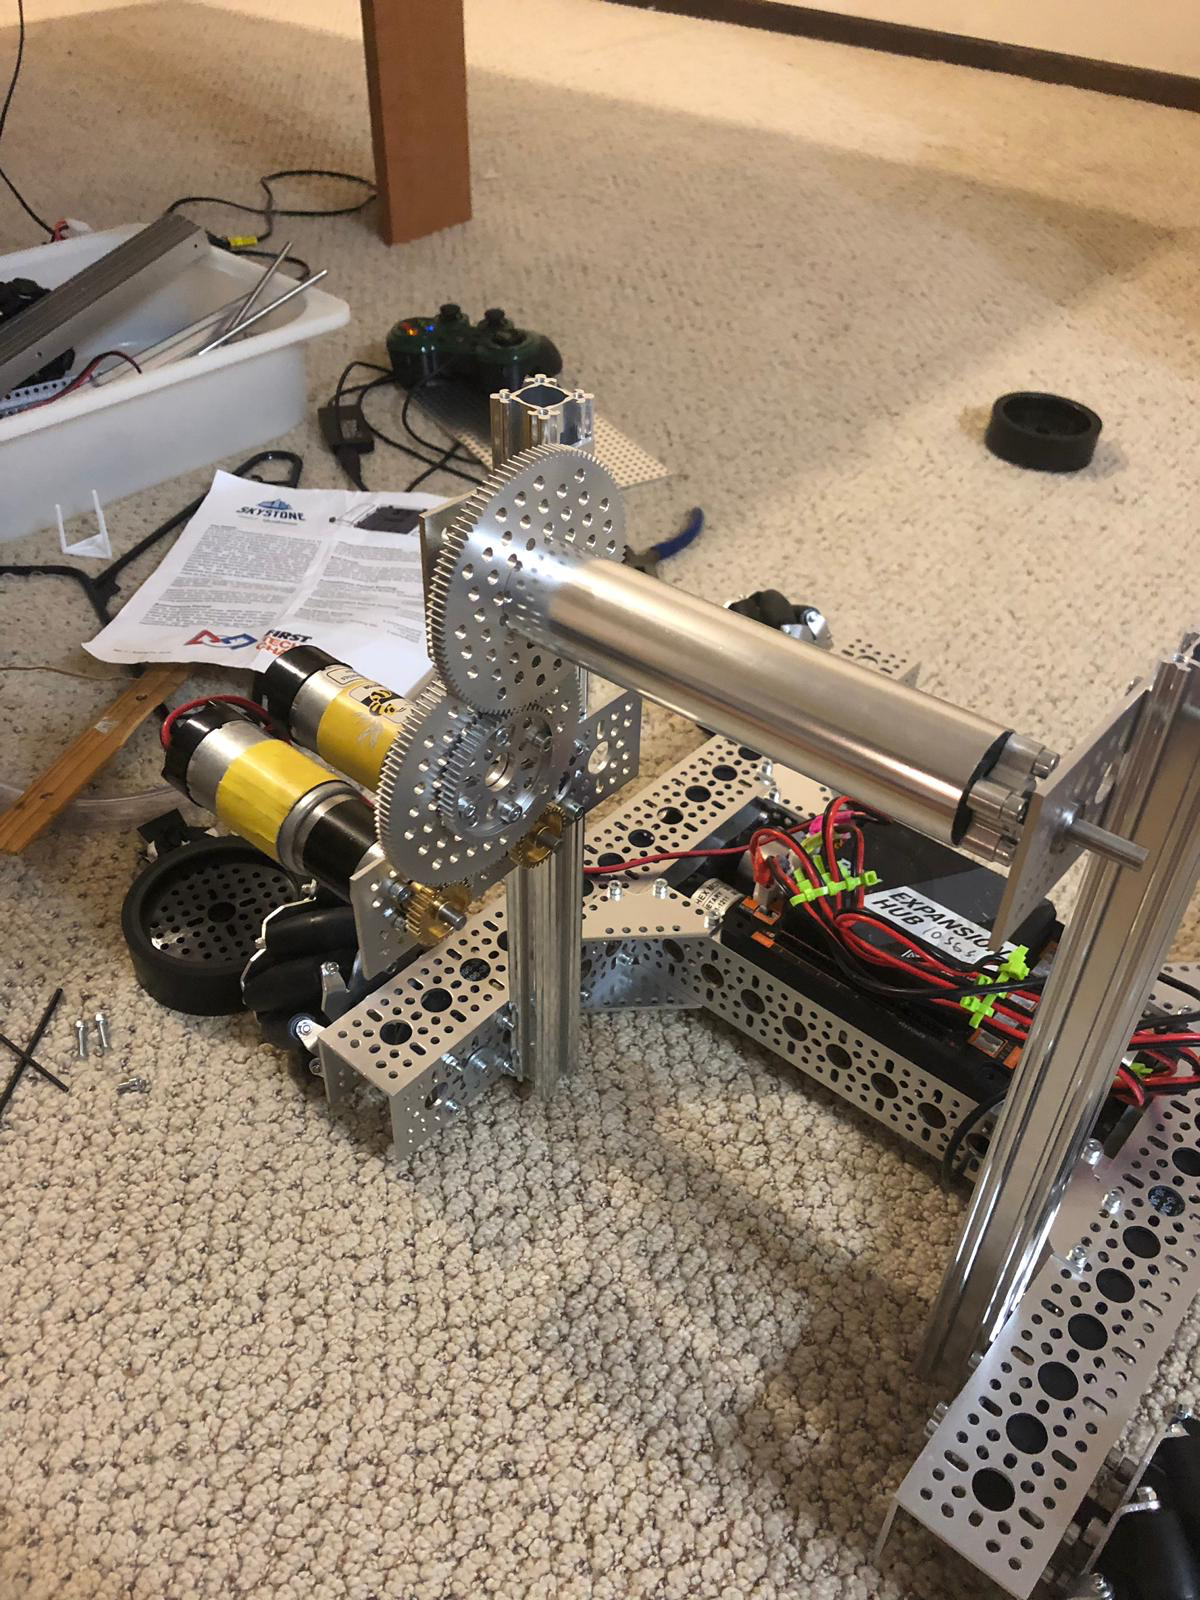
\includegraphics[width=.5\textwidth]{Images/9-8robot.png}
    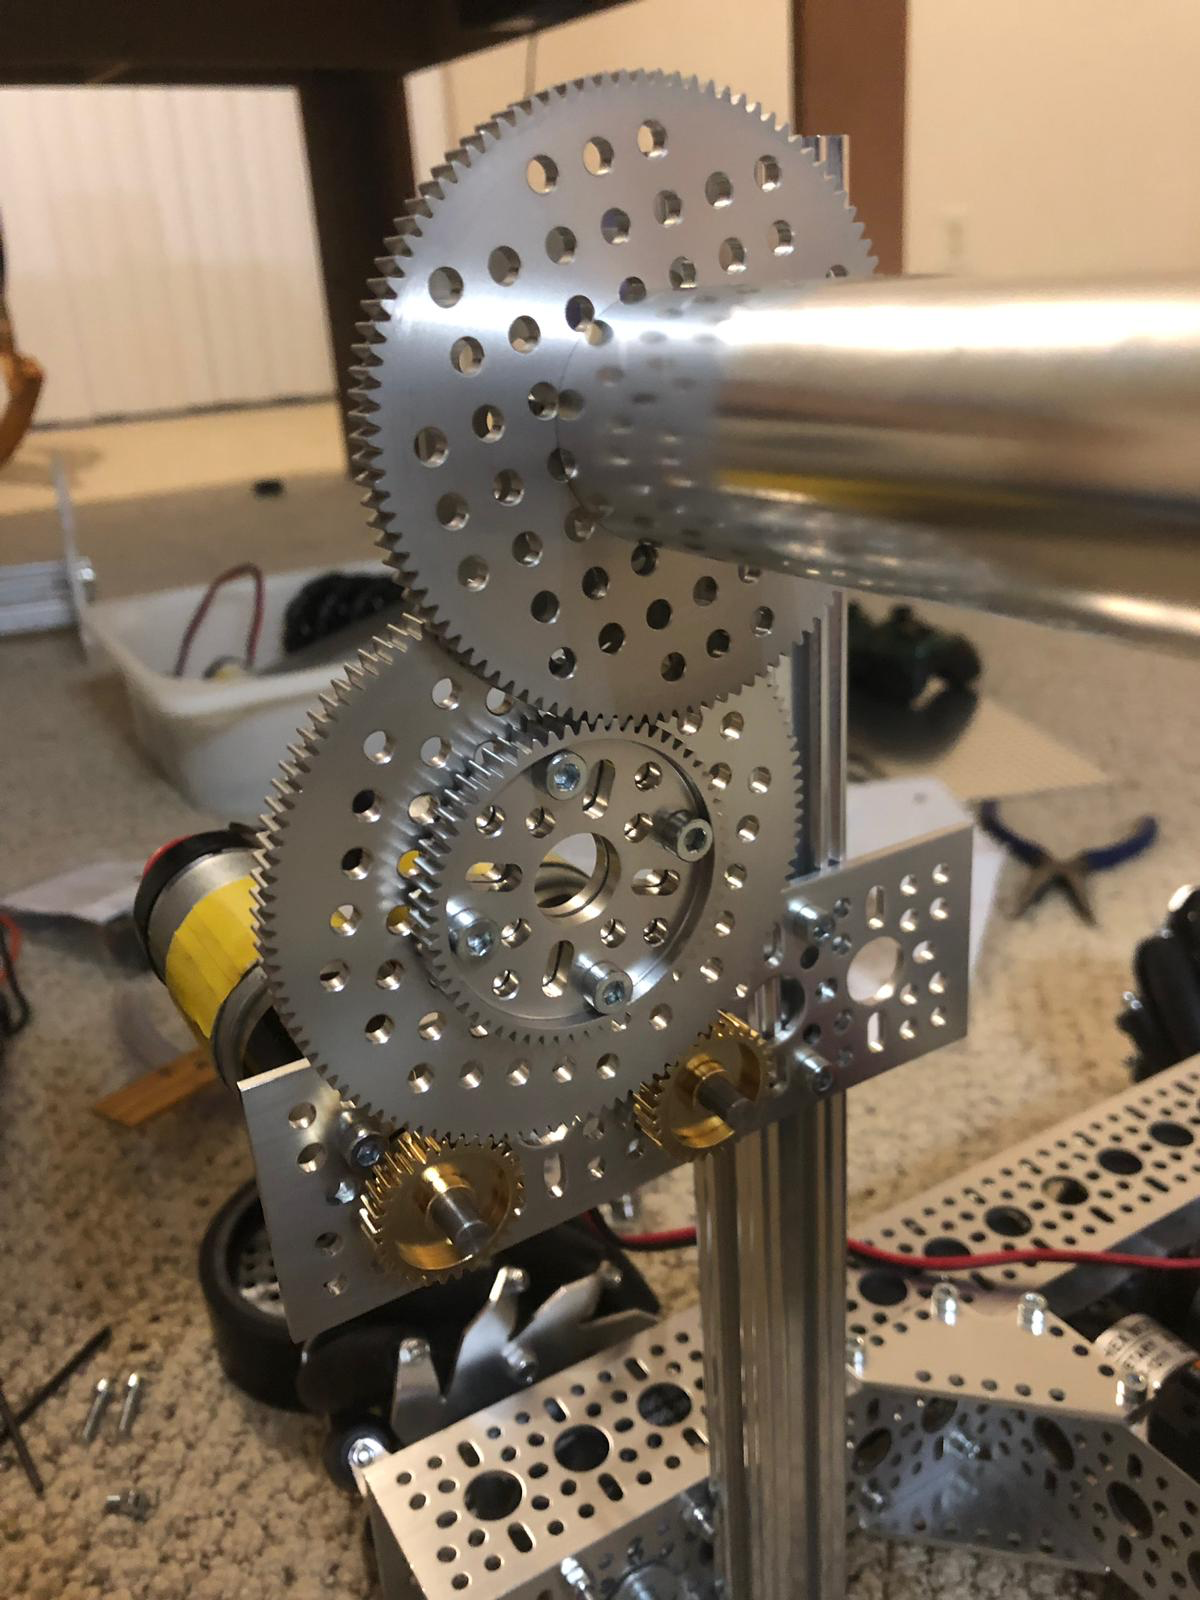
\includegraphics[width=.5\textwidth]{Images/9-8gears.png}\\
    Our robot after Day 1
\end{center}
\newpage

\infoBox{Chain Bar}{}

\practicenotes{9/9/19 3:30pm - 9:00pm}{Sprint 0 (Robot in 3 Days) - Practice}{Josh, Julia, Michael, Oliver, Ori, Rachel, Sarah}{
    Building\\\\
    We bought polycarbonate to use for the arm and the intake. We chose polycarbonate because it is lightweight and flexible, meaning it is resistant to breaking. Oliver cut and drilled the polycarbonate and axles for the intake, with help from Sarah and Josh. Oliver also assembled the gearboxes for the intake using the parts cut and gears that were 3D printed. Ori assembled the gear box for the chain bar and attached motors to the gearbox with help from Rachel.\\\\
    Written by: Rachel and Josh
}
\begin{center}
    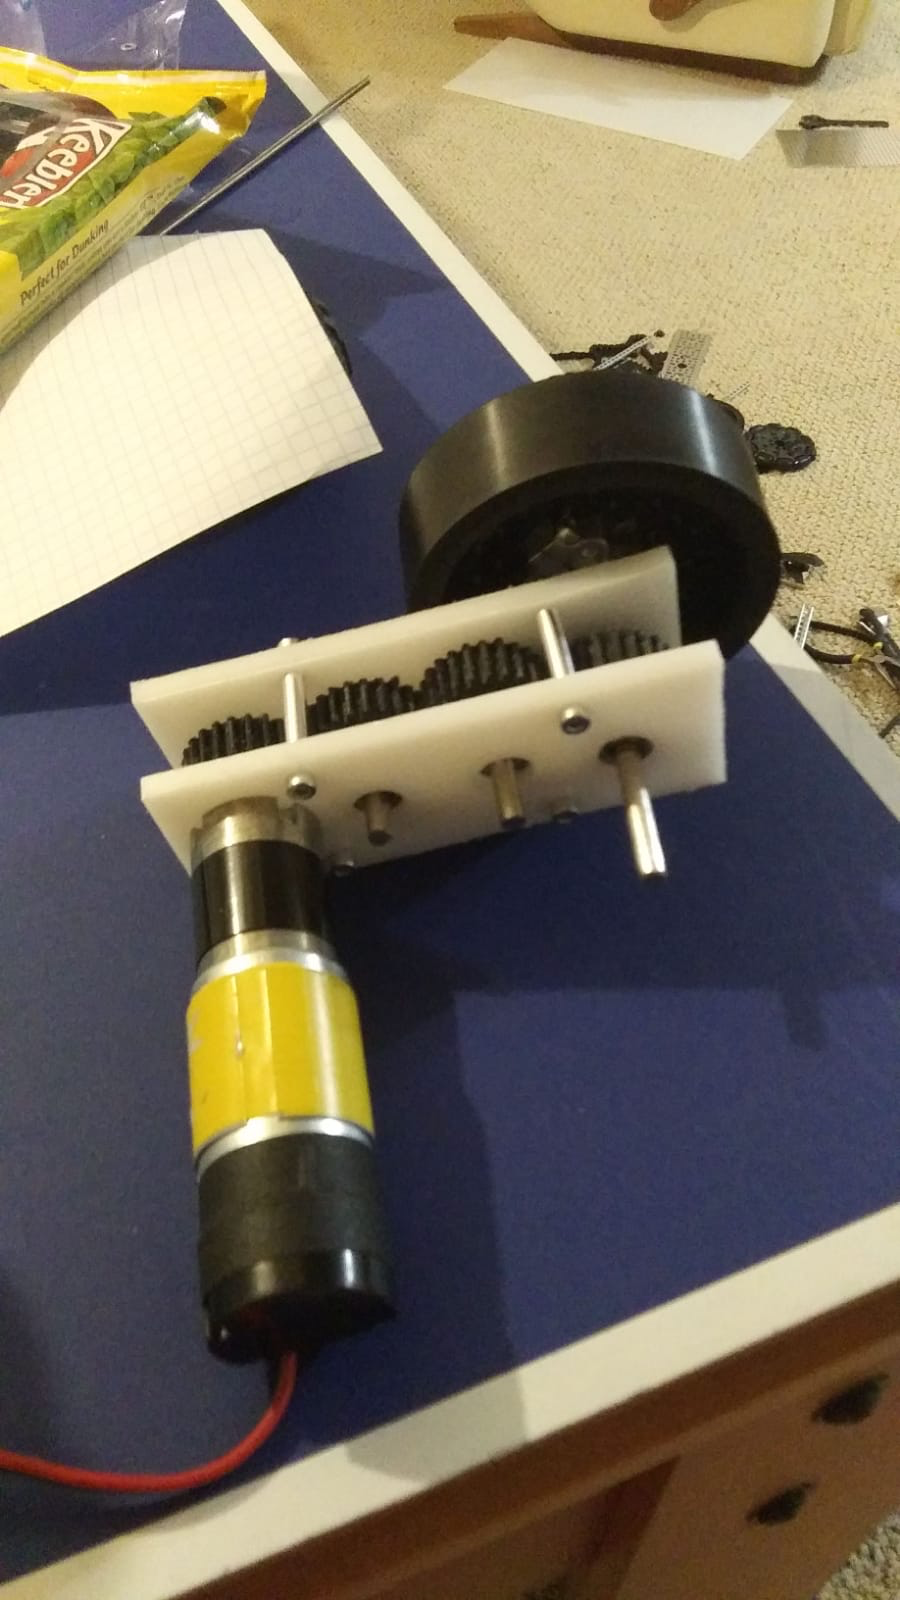
\includegraphics[width=.4\textwidth]{Images/9-9intake.png}
    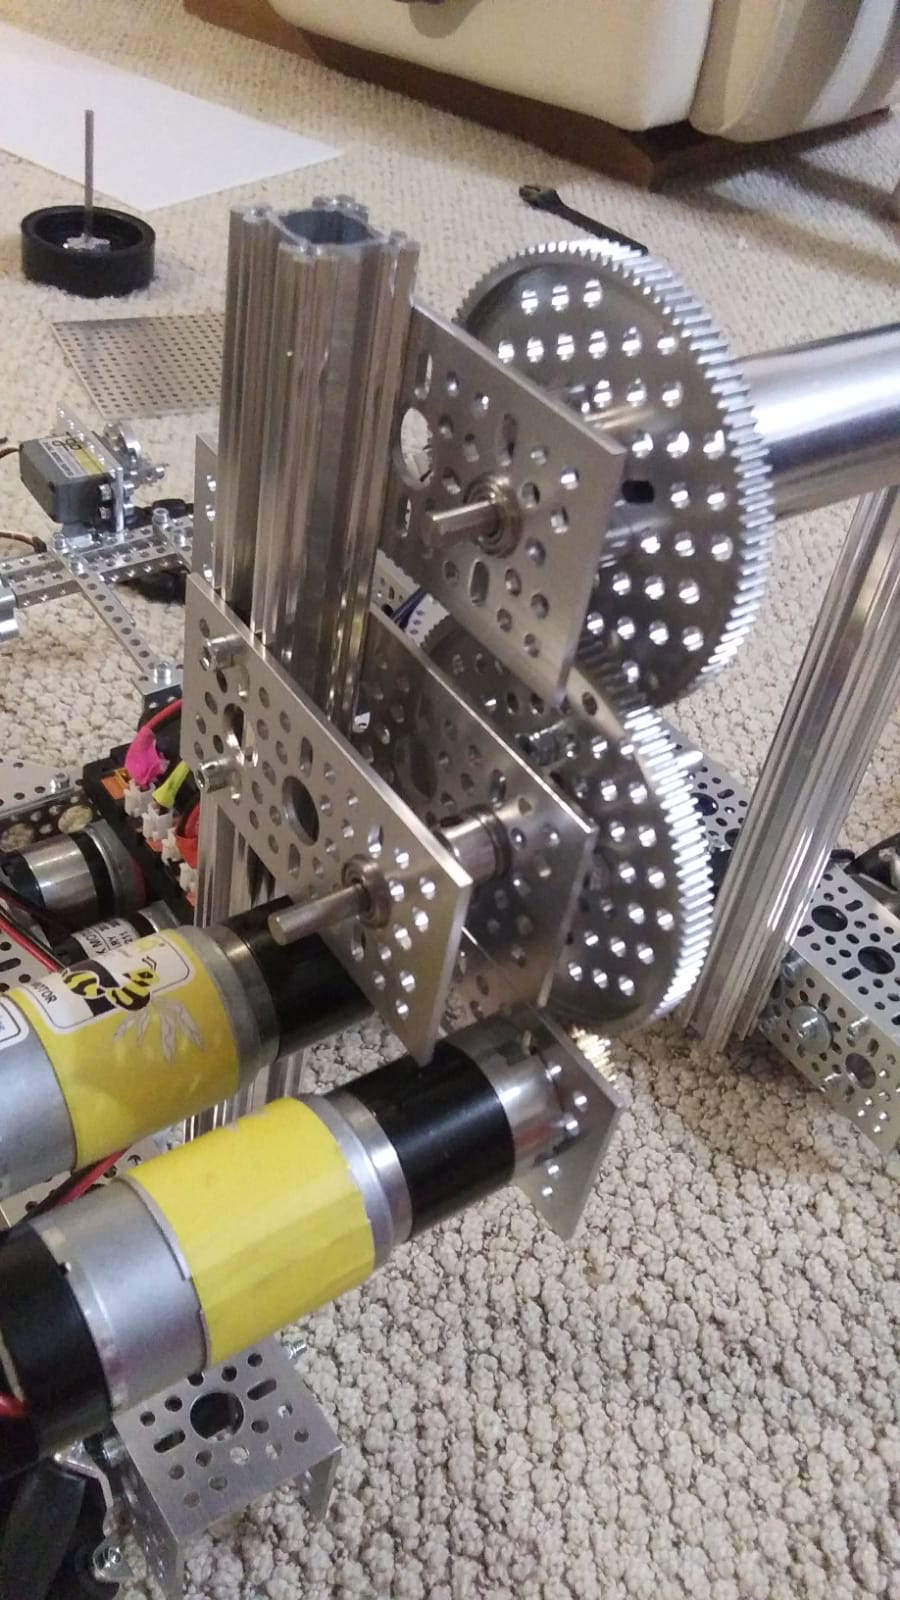
\includegraphics[width=.4\textwidth]{Images/9-9gears.png}\\
    The intake, gears, and claw at the end of Day 2\\
    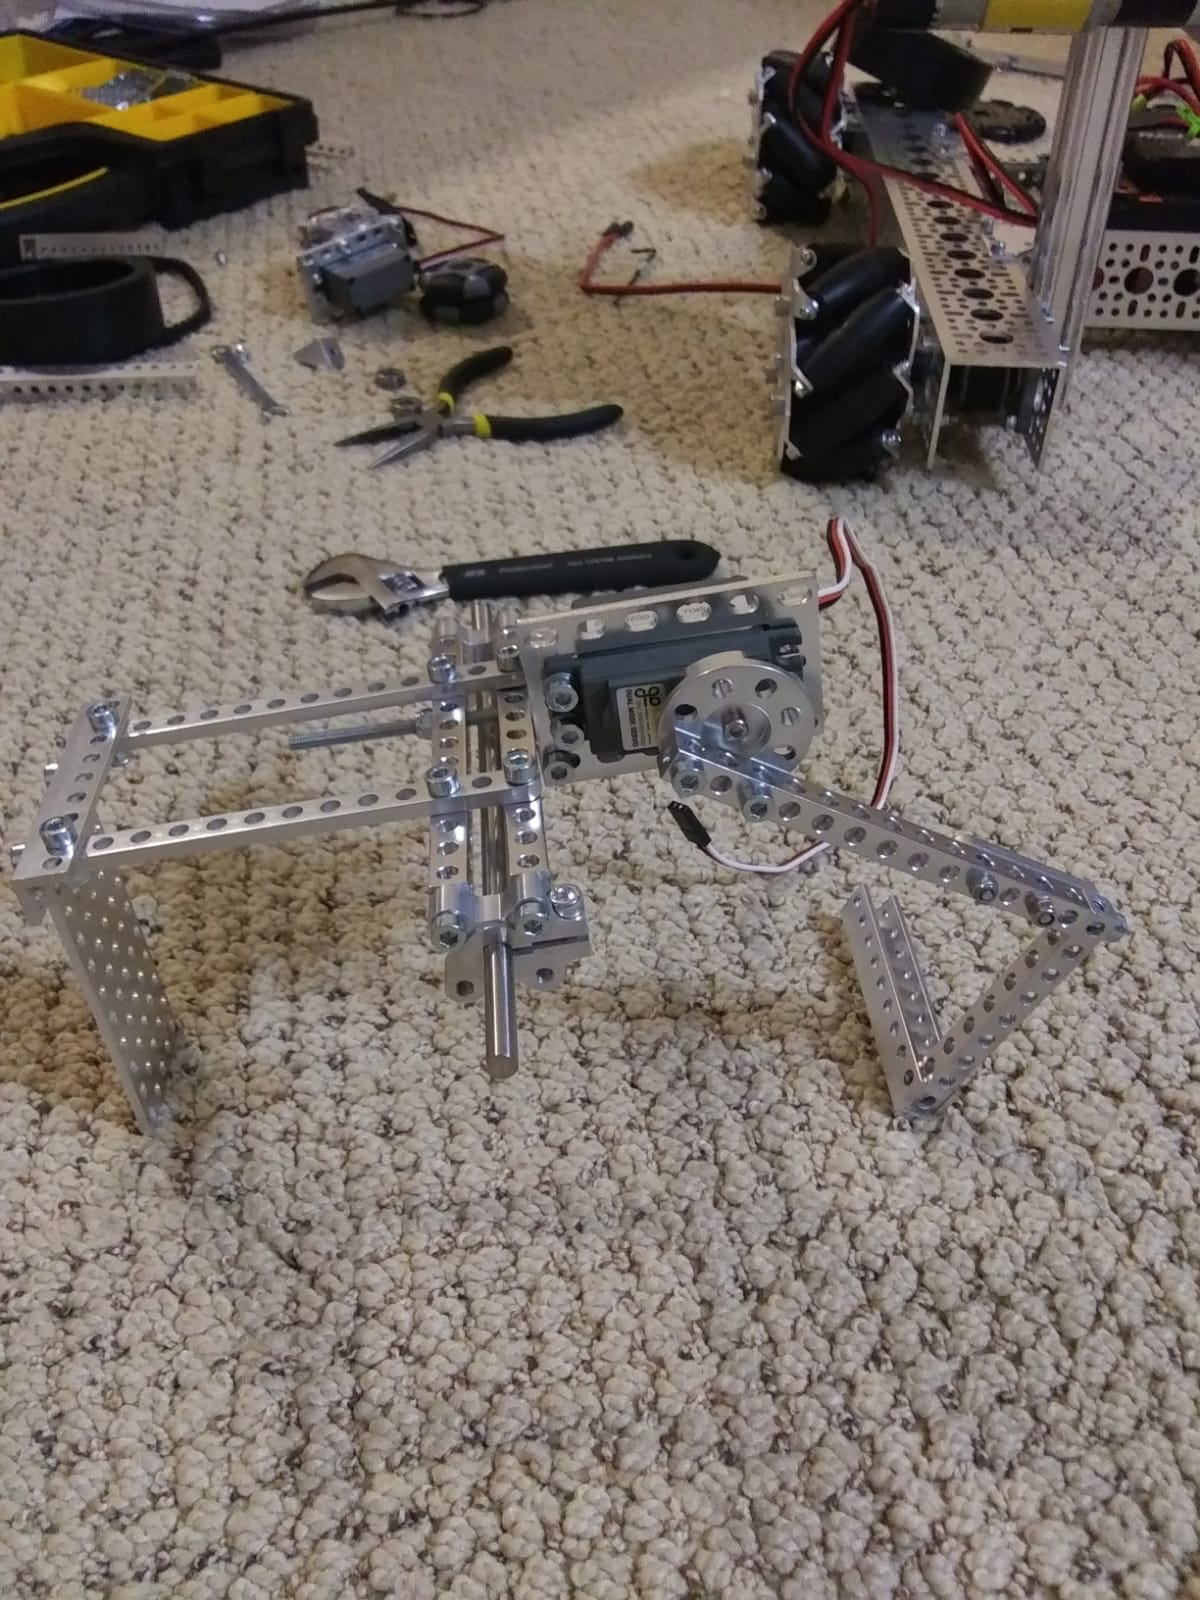
\includegraphics[width=.5\textwidth]{Images/9-9claw.png}
\end{center}
\newpage

\practicenotes{9/10/19 4:30pm - 9:00pm}{Sprint 0 (Robot in 3 Days) - Practice}{Julia, Oliver, Ori, Rachel}{
    Building\\\\
    Oliver is drilling holes in the arm to attach it to the robot and intake. He is also working on the second half of the intake (we made the first half yesterday). Ori is getting the chain bar to work, adding the belt, and attaching the claw. Julia is helping by adding a support beam to the arm, which is helpful because the length of the arm. Ori added the belt to the chain bar, which will ensure that the claw remains at the same angle to the ground the entire time so that the Stones will be correctly aligned and easy to stack.\\\\
    Written by: Rachel
}
\practicenotes{9/11/19 3:30pm - 9:00pm}{Sprint 0 (Robot in 3 Days) - Practice}{Julia, Michael, Oliver, Ori, Rachel, Sarah}{
    Building\\\\
    The entire team worked on attaching all of the components of the robot. We were working throughout a lot of the day but were at different practice sites, as there was a club-wide meeting at 6. Ori changed the location of the top pulley of the belt drive so that the belt would be parallel to the side of the robot instead of slanted, which was a source of errors when we tested it yesterday. Oliver and Michael attached the two halves of the intake, and added the springs. The springs pull the intake in, but there is also a metal piece that stops the intake arms from coming in too much. The springs allow the arms to move enough to intake the Stones effectively. The rest of the team worked on wiring, attaching the REV hubs, and attaching other small components. We were able to test the intake and the claw by the end of the day, and it worked well with our makeshift Stone. We will have the field and real stones to test our robot with sometime next week.\\\\
    Written by: Rachel
}

\practicenotes{9/13/19 6:00pm - 9:00pm}{Sprint 0 (Robot in 3 Days) - Practice}{Josh, Julia, Ori, Michael, Sarah, Oliver}{
    Outreach\\\\
    Michael, Ori and Oliver went to Michael's house before practice to film a robot reveal for RI3D. They shot videos of the robot moving, intaking and placing a stone and playing chess.\\\\
    Written by: Josh
}


\end{document}